\section{Theoretical Analysis}
\label{sec:analysis}

In this section we will detail the theoretical study of the Amplifier Circuit conducted during this lab. The circuit was divided into two seperate ones: the gain stage and the outrput stage. The first one increased the gain, but it had a drop of current considered undesirable due to the output impedance. The latter one corrects this effect while having a gain near one, as to not decrease the voltage previously gained.\\
The entire circuit can be seen in the following image:\\



\begin{figure} [!htb] 
  \minipage{0.9\textwidth}
  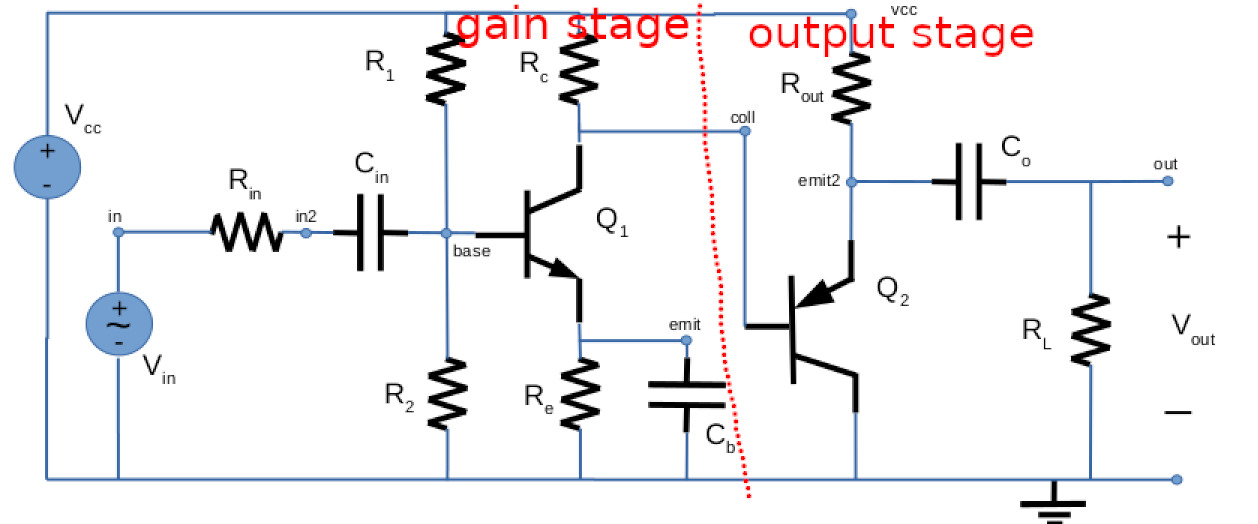
\includegraphics[width=\linewidth]{circuitsep.jpeg}
  \caption{The amplifier stages}
  \label{fig:stage}
  \endminipage\hfill
\end{figure}


One must note that Vin and Rin constitute the thevenin equivalent of the circuit to which the amplifier is connected.\\
The capacitator connected to Rin will enforce that only the AC part of the voltage is taken into account. The DC part is suplied by a constant 12V voltage source Vcc. With this arquitecture, we can ensure that the transistors are in foward active region (FAC), for the Vcc will force an voltage drop bigger than the one necessary for that mode of operation.\\
It was used an Operanting Point analysis where the DC component of the current and voltage is taken into account, but not the AC one, followed by an Incremental Analysis where the AC component of the current and voltage is taken and where a linear model of the transistor is assumed. By adding the results, we can obtain a solution for the circuit, thereby obtaining the values necessary to compute the theoretical gain of the amplifier and the various impedances, such as the input and output ones.
The analysis can be divided into the following particular smaller analysis:
\begin{itemize}
	\item Operating Point analysis for the gain stage;
	\item Incremental analysis for the gain stage;
	\item Calculation of the gain for the gain stage;
	\item Operanting Point analysis for the output stage;
	\item Incremental analysis for the output stage;
	\item Calculation of the gain for the output stage;
	\item Calculation of the input and output inpedances;
\end{itemize}

To calculate the OP of each stage, it was considered the following circuits for each stage:

\begin{figure} [!htb] 
  \minipage{0.9\textwidth}
  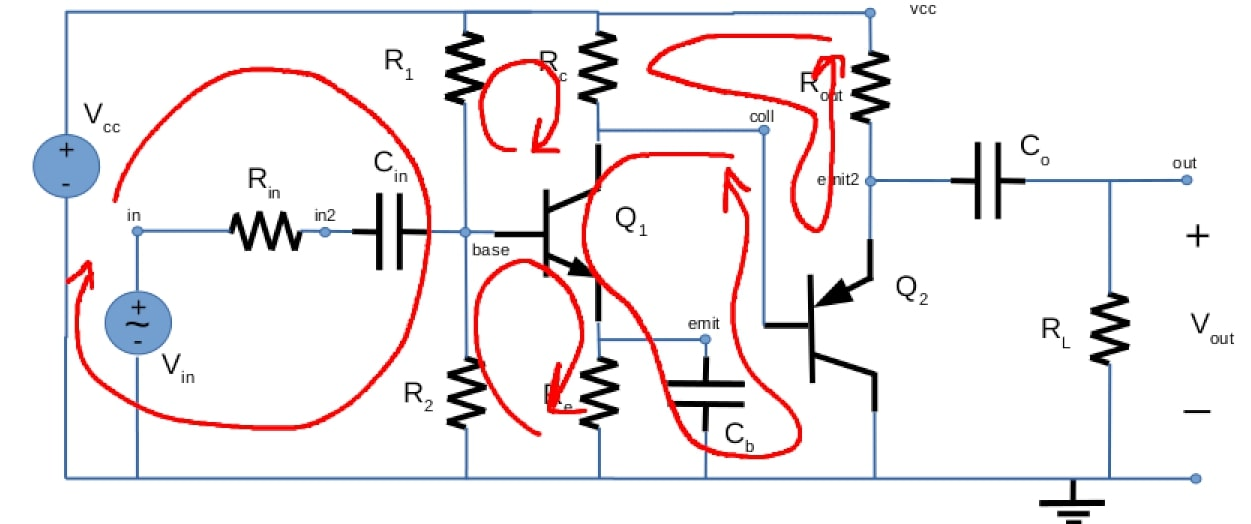
\includegraphics[width=\linewidth]{malhas.jpeg}
  \caption{Meshes for OP analysis}
  \label{fig:mesh}
  \endminipage\hfill
\end{figure}


It was used the mesh method in conjuction with the Ebers-Moll bipolar npn transistor model in order to calculate the currents in each mesh and the voltage drops between nodes. With this, it was possible to calcule the DC component of the output volltage.\\

The transistor was modeled as follows:\\

\begin{equation}
 g_{m} = I_{C}/V_{T}
 \label{}
\end{equation} 

\begin{equation}
 r_{\pi}= {\beta}_{F}/g_{m}
   \label{}
\end{equation} 

\begin{equation}
  r_{o}= V_{A}/I_{C}
  \label{}
\end{equation} 

To calculate the incremental stage, it was considered the following incremental model of the transistor:\\



\begin{figure} [!htb] 
  \minipage{0.9\textwidth}
  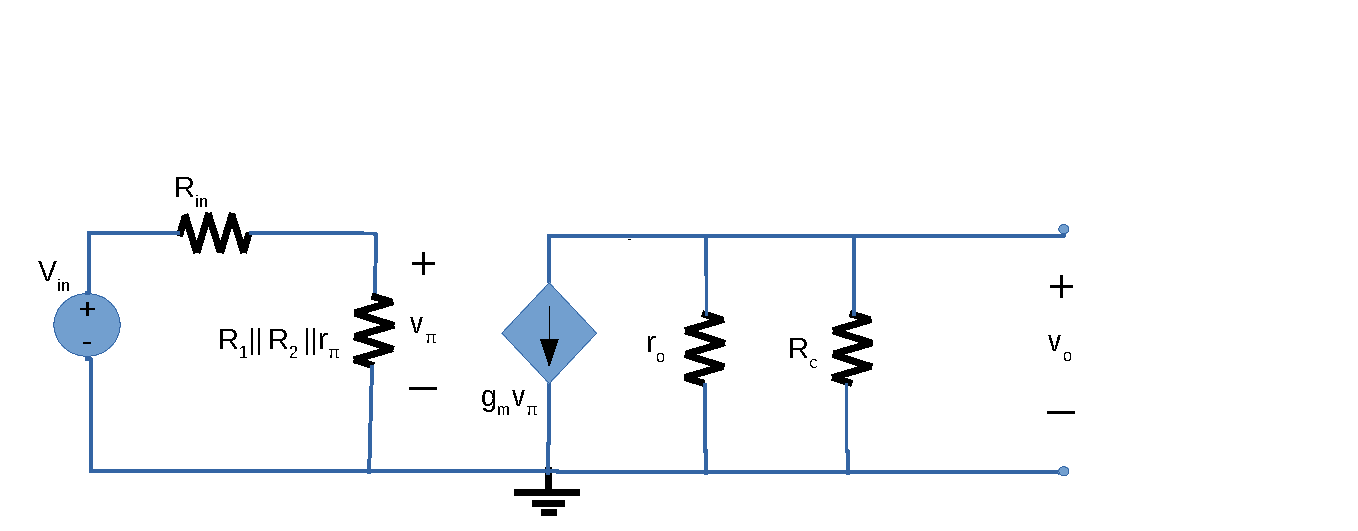
\includegraphics[width=\linewidth]{incrementalgain.pdf}
  \caption{Incremental Gain}
  \label{fig:theoplots}
  \endminipage\hfill
\end{figure}



\begin{figure} [!htb] 
  \minipage{0.9\textwidth}
  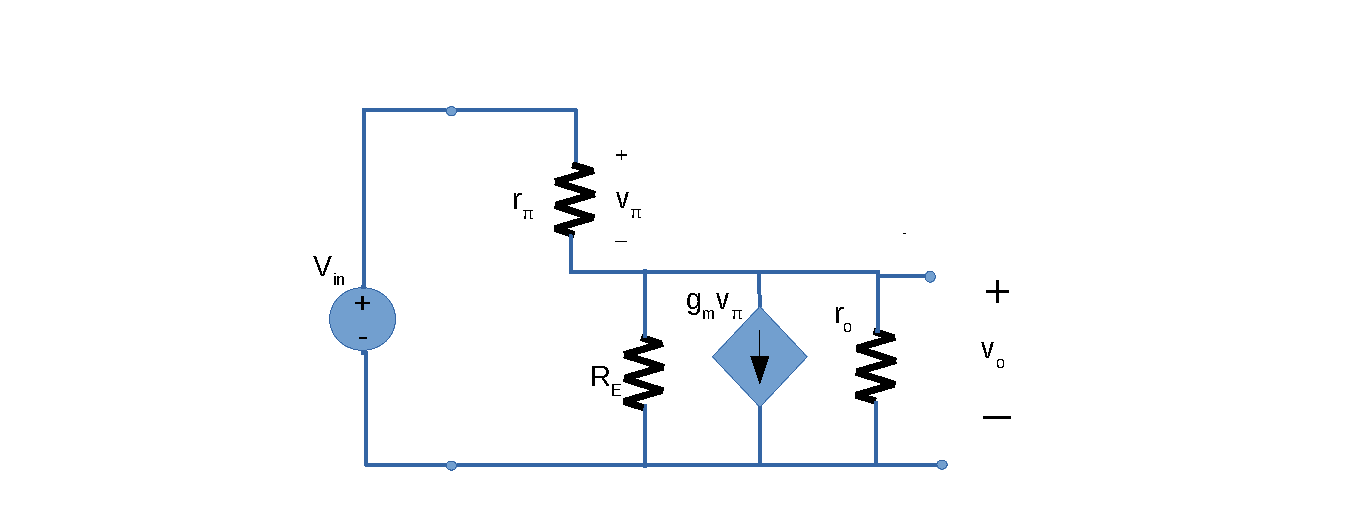
\includegraphics[width=\linewidth]{incrementaloutput.pdf}
  \caption{Incremental Output}
  \label{fig:theoplots}
  \endminipage\hfill
\end{figure}

\FloatBarrier

By using the mesh method, it was possible to calculate the AC component for the output voltage.\\
The total voltage for each frequencie is equal to the sum of the AC with the DC component.\\

This analysis was repeated for various frequencies of Vin (10 equally spaced frequencies per decade), and the results were ploted on a dB scale.
The calculation of the overall gain was obtained by multiplying the gain of each stage. The results can be observed in the following graphs:\\ 




\begin{figure} [!htb] 
  \minipage{0.9\textwidth}
  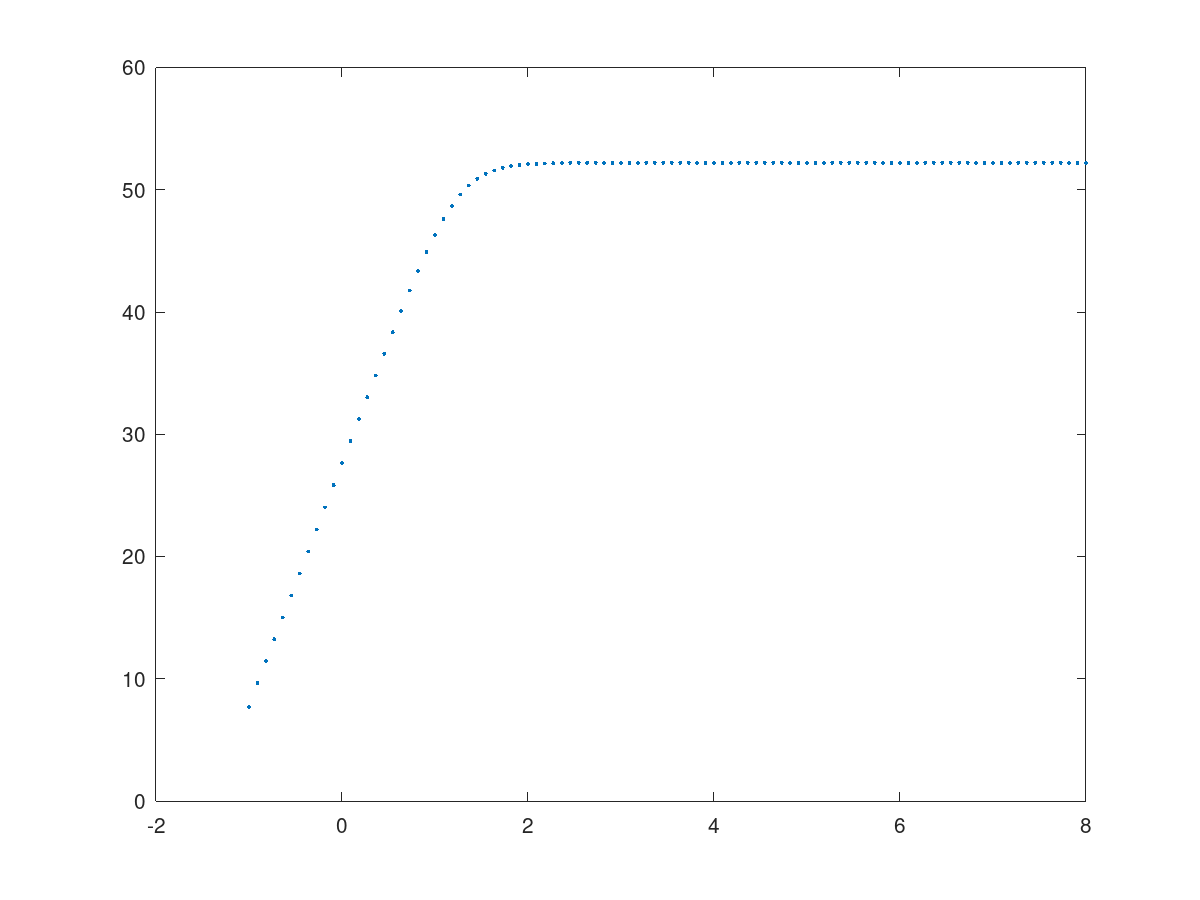
\includegraphics[width=\linewidth]{GAINVERDADEIRO.png}
  \caption{Gain with R3=0}
  \label{fig:theoplots}
  \endminipage\hfill
\end{figure}


\begin{figure} [!htb] 
  \minipage{0.9\textwidth}
  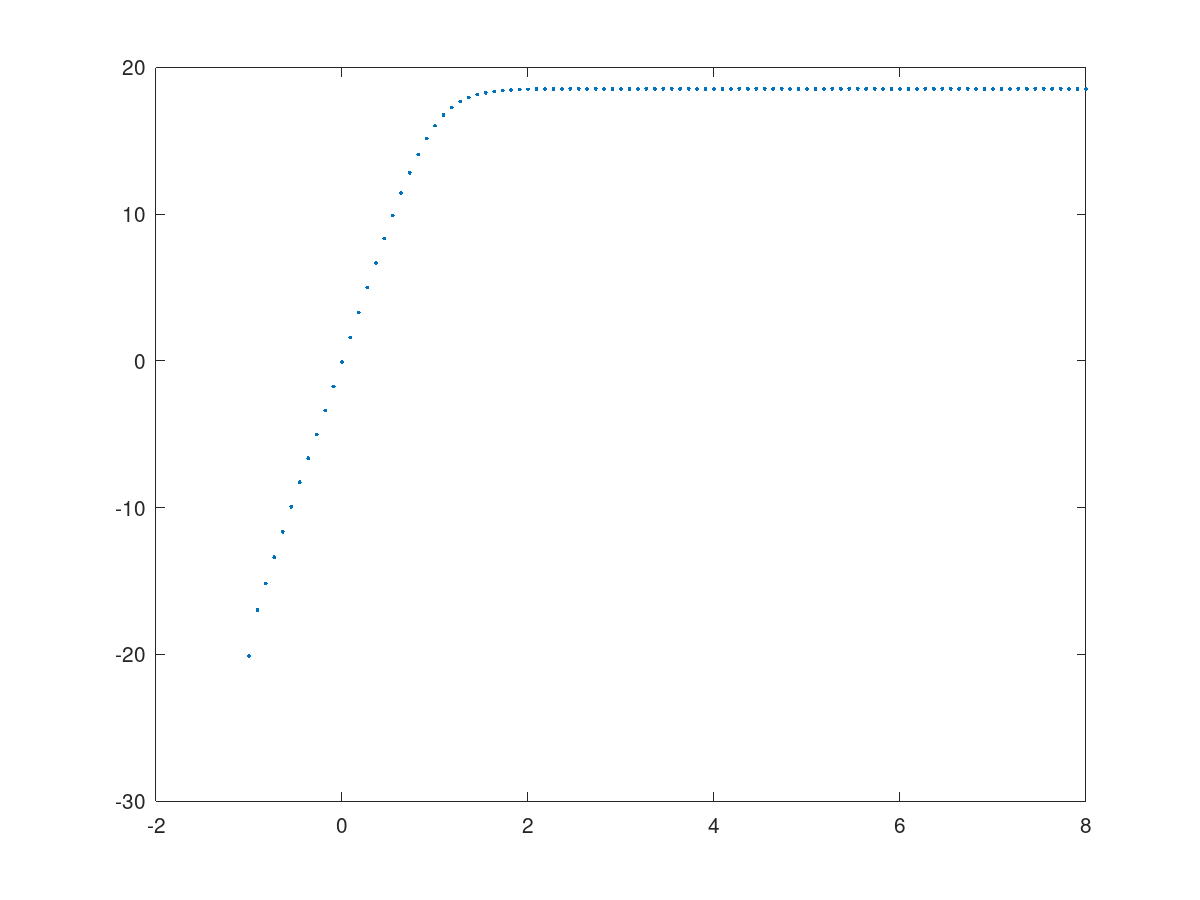
\includegraphics[width=\linewidth]{GAIN_Exprimental_R3_a_0.png}
  \caption{Gain with abitrated values}
  \label{fig:theoplots}
  \endminipage\hfill
\end{figure}

\FloatBarrier




